\documentclass[a4paper,8pt,titlepage]{scrbook}

\usepackage[T1]{fontenc}
\usepackage[utf8]{inputenc}
\usepackage[ngerman]{babel}
\usepackage{hyperref}
\usepackage{tabularx}
\usepackage{wrapfig}
\usepackage{amsmath}
\usepackage{amssymb}
\usepackage{graphicx}
\usepackage{listings}
\usepackage{listings_mips}
\usepackage{listings_vhdl}
\usepackage[ruled,vlined]{algorithm2e}
\usepackage{esdiff}
\usepackage{float}
\usepackage{geometry}
\geometry{left=2cm,right=2cm,top=2cm,bottom=2cm,bindingoffset=10mm}
\restylefloat{table}

\title{Rechnerstrukturen am Karlsruher Institut für Technologie}
\date{August 2019}
\author{Maximilian Heß, überarbeitet durch Carolin Beer}

Zusammenfassung der Vorlesung "`Rechnerstrukturen"' aus dem Sommersemester 2019.\footnote{\url{https://capp.itec.kit.edu/teaching/rs/}}


\begin{document}
\maketitle
\tableofcontents
\setcounter{tocdepth}{2}
\setcounter{secnumdepth}{2}
\chapter{Grundlagen}

\section{Einführung}
	Entwurf einer Rechneranlage: Ingenieurmäßige Aufgabe der Kompromissfindung zwischen Zielsetzung, Randbedingungen, Gestaltungsgrundsätzen und Anforderungen.

\section{Entwurf von Rechneranlagen - Entwurfsfragen}
	\paragraph{Heutige Kennzahlen}
		\begin{itemize}
			\item Höchstleistungsrechner: Exa-FLOPs ($10^{18}$)
			\item Intel Skylake-Prozessoren: 8 Mrd. Transistoren
			\item Strukturbreite: 10nm 
		\end{itemize}

	\paragraph{Prozessortypen}
		\begin{itemize}
			\item Multicore/Manycore
			\item Anwendungsspezifisch, bspw. Google TPUs 
		\end{itemize}

	\paragraph{Zielsetzung}
		\begin{itemize}
			\item \textbf{Einsatzgebiet}
			\begin{itemize}
				\item \textbf{Desktop Computing}
				\begin{itemize}
					\item PCs bis Workstations (\$1000 - \$10.000)
					\item Günstiges Preis-/Leistungsverhältnis
					\item Ausgewogene Rechenleistung für ein breites Spektrum von (interaktiven) Anwendungen
				\end{itemize}
				\item \textbf{Server}
				\begin{itemize}
					\item Rechen- und datenintensive Anwendungen
					\item Hohe Anforderungen an die Verfügbarkeit und Zuverlässigkeit
					\item Skalierbarkeit
					\item Große Dateisysteme und Ein-/Ausgabesysteme
				\end{itemize}
				\item \textbf{Eingebettete Systeme}
				\begin{itemize}
					\item Mikroprozessorsysteme, eingebettet in Geräte und daher nicht unbedingt sichtbar
					\item Sind auf spezielle Aufgaben zugeschnitten (hohe Leistungsfähigkeit, Spezialprozessoren)
					\item Breites Preis-/Leistungsspektrum
					\item Echtzeitanforderungen
					\item Abwägung der Anforderungen an Rechenleistung, Speicherbedarf, Kosten, Energieverbrauch, etc.
				\end{itemize}
			\end{itemize}
			\item \textbf{Anwendungsbereich}
			\begin{itemize}
				\item Technisch-wissenschaftlicher Bereich: Hohe Anforderungen an die Rechenleistung, insbesondere Gleitkommaverarbeitung
				\item Kommerzieller Bereich: Datenbanken, WEB, Suchmaschinen, Optimierung von Geschäftsprozessen, etc.
				\item Eingebettete Systeme: Verarbeitung digitaler Medien, Automatisierung, Telekommunikation, etc.
			\end{itemize}
			\item \textbf{Rechenleistung}
			\begin{itemize}
				\item Ermittlung über Benchmarks
				\item Maßzahlen für die Operationsleistung: \textit{MIPS} oder \textit{MFLOPS}
				\item \(MFLOPS = \frac{\texttt{Anzahl ausgeführter Gleitkommainstruktionen}}{10^6 \cdot \texttt{Ausführungszeit}}\)
			\end{itemize}
			\item Verfügbarkeit
			\item \textbf{Zuverlässigkeit}
			\begin{itemize}
				\item Bei Ausfällen von Komponenten muss ein betriebsfähiger Kern bereit sein
				\item Verwendung redundanter Komponenten
				\item Bewertung der Ausfallwahrscheinlichkeit mittels stochastischer Verfahren
				\item Definition Verfügbarkeit: Wahrscheinlichkeit, ein System zu einem beliebigen Zeitpunkt fehlerfrei anzutreffen
			\end{itemize}
		\end{itemize}

	\paragraph{Randbedingungen}
		\begin{itemize}
			\item Technologische Entwicklung: Mikrominiaturisierung setzt sich fort, beispielsweise Verkleinerung der Strukturbreiten sowie Erhöhung der Integrationsdichte (Anzahl der Transistoren verdoppelt sich alle 18 Monate)
			\item Größe
			\item Geld
			\item \textbf{Energieverbrauch}
			\begin{itemize}
				\item Mobile Geräte: Verfügbare Energiemenge durch Batterien und Akkumulatoren ist begrenzt \(\rightarrow\) möglichst lange mit der vorhandenen Energie auskommen
				\item Vermeiden von Überhitzungen
				\item Green IT: Niedriger Energieverbrauch, ökologische Produktion, einfaches Recycling
			\end{itemize}
			\item Umwelt
		\end{itemize}

	\paragraph{Sonstiges}
		\begin{itemize}
			\item Gestaltungsgrundsätze: Modularität, Sparsamkeit, Fehlertoleranz, etc.
			\item Anforderungen: Kompatibilität, Betriebssystemanforderungen, Standards, etc.
		\end{itemize}

\paragraph{Trends in der Rechnerarchitektur: Herausforderungen}
Weltweite Forschungsaktivitäten bzgl. ExaScale-Rechner
\begin{itemize}
	\item Verlustleistung: Überträgt man heutige (Stand 2010) Höchstleistungsrechner in den Exascale-Bereich, hätte man eine Verlustleistung von etwa 40 GW (diese kann allerdings höchstens 20-40 MW betragen)
	\item Hauptspeicher (DRAM), permanenter Speicher: Kapazität und Zugriffsgeschwindigkeit muss mit der Rechengeschwindigkeit mithalten
	\item Zuverlässigkeit und Verfügbarkeit
	\item Parallelität und Lokalität
\end{itemize}


\section{Effizienter Entwurf --- Grundlagen}
	\begin{itemize}
		\item Mobile Geräte: Verfügbare Energiemenge durch Batterien und Akkus begrenzt \(\rightarrow\) vorhandene Energie möglichst lange ausnutzen sowie Vermeidung von Überhitzung
		\item HPC: Hohe Temperaturen begrenzen die Verarbeitungsgeschwindigkeit und die beeinflussen die Zuverlässigkeit
	\end{itemize}

	\paragraph{CMOS-Schaltung}
		\begin{itemize}
			\item MOSFET: Je nach Spannung am Gate und dem daraus resultierenden Feld im Kanal können Ladungsträger den Kanal passieren oder nicht. Extrem niedrige Stromaufnahme im Ruhezustand
			\item \textbf{Leistungsaufnahme}
			\begin{itemize}
				\item \(P_{total} = P_{switching} + P_{shortcircuit} + P_{static} + P_{leakage}\)
				\item Statischer Leistungsverbrauch: \(P_{static}\) sowie Leistungsverbauch $(P_{leakage}$ bei Kriechströmen
				\item Verbrauch bei Zustandsänderung: \(P_{switching}=C_{eff}*V_{dd}^2*f\) sowie Verbrauch während des Übergangs am Ausgang, wenn sich die Eingänge ändern \(P_{shortciruit}=I_{mean}*V_{dd}\) 
				\item Höhere Frequenzen erfordern steilere Taktflaken \(\rightarrow\) schnelleres Laden von \(C_{eff}\) \(\rightarrow\) höhere Versorgungsspannung 
				\item \(P \sim f und P \sim V_{dd}^2\) aber da $f \sim V_{dd}^2 \Rightarrow P \sim V_{dd}^3 $ und $P \sim f^3$
				\item Energieverbrauch pro Aufgabe ist unabhängig von Frequenz, bzw. sogar negativ korreliert wegen statischer Ströme		
			\end{itemize}
			\item \textbf{Schaltwahrscheinlichkeit}
			\begin{itemize}
				\item \(\mathbb{P}_{Schalt} = 2 \cdot \mathbb{P}_{Ausgang(1)} \cdot (1-\mathbb{P}_{Ausgang}(1))\)
				\item \(\mathbb{P}_{Ausgang}(1) = \mathbb{P}_{Eingang1}(0) \cdot \mathbb{P}_{Eingang2}(1) + \mathbb{P}_{Eingang1}(1) \cdot \mathbb{P}_{Eingang2}(0)\)
			\end{itemize}
	\end{itemize}

	\paragraph{Kosten von Prozessoren}
		\begin{itemize}
			\item \textbf{Ziel}
			\begin{itemize}
				\item Leistungsaufnahme senken ohne Verarbeitungsgeschwindigkeit zu beeinträchtigen
				\item Optimierung der Systemarchitektur
				\item Spezialisierte Prozessorkerne/Multicore-CPUs, die Parallelverarbeitung erlauben, verwenden
			\end{itemize}
			\item \textbf{Kosten} Proportional zu $\sqrt{A_{Wafer}}$, Chipfläche wird durch Entwickler beeinflusst
			\begin{itemize}
				\item $C_{Die}=\frac{C_{Wafer}}{\frac{\texttt{\#Dies}}{Wafer}*Ausbeute}$
				\item $\texttt{\#Dies}=\frac{\pi*r_{Wafer}^2}{A_{Die}}-\frac{2\pi*r_{Wafer}}{\sqrt{2*A_{Die}}}$
				\item $\texttt{Ausbeute}=\frac{\texttt{Ausbeute}_{Wafer}}{(1+\texttt{Defekte})^N}$
			\end{itemize}
		\end{itemize}

\section{Einführung in den Entwurf eingebetteter Systeme}
	\paragraph{Die Hardware-Beschreibungssprache VHDL}
		\begin{itemize}
			\item Standardisierte Hardware-Beschreibungssprache: Die verschiedenen Schaltungsbeschreibungen des gesamten Entwurfsablaufs können dargestellt werden - von der algorithmischen Spezifikation bis hin zu realisierungsnahen Strukturen
			\item Eingesetzt zum ASIC- und FPGA-Entwurf
			\item Bei synchroner Zuweisung werden Änderungen abhängig von einem Takt und den Eingangssignalen geändert. Bei asynchroner Zuweisung unabhängig und unmittelbar (nach einer gewissen Schaltzeit)
			\item Automatischer Synthesewerkzeuge: Flexibilität, weniger fehleranfällig. Dafür Randbedingungen schwer einzuhalten und Ergebnisse oft schlechter als bei manuellem Entwurf
		\end{itemize}
	\paragraph{Chip-Entwurf(Top-Down)}
		\begin{itemize}
			\item Grundlage des Entwurfs ist die Spezifikation der Schaltung: Gewünschtes Verhalten; Schnittstellen; Vorgaben bzwgl. Geschwindigkeit, Kosten, Fläche oder Leistungsverbrauch
			\item Entwurfsschritte: Verhaltensspezifikation, High-Level-Synthese, RT-Beschreibung, Logik-Synthese, Gatterbeschreibung, Layout-Synthese, Geometriegebschreibung, Fertigung
			\item \textbf{Hauptbestandteile} 
			\begin{itemize}
				\item ENTITY: Schnittstellen
				\item ARCHITECTURE: Verhalten
				\item CONFIGURATION: Weist COMPONENT-Instanzen zu ENTITY und ARCHITECTURE zu.
			\end{itemize} 
			\item Signale zur Kommunikation zwischen Instanzen untereinander oder mit Schnittstellen der äußeren Hülle (Entity)
			\item Schnittstellendefinition eines MODULS\\\\
			\begin{minipage}{\linewidth}
				\begin{lstlisting}[frame=single,numbers=left,mathescape,language=VHDL,tabsize=4]
	ENTITY blinklicht IS
		PORT(
			clk: IN Std_Logic;
			reset: IN Std_Logic;
			led: OUT Std_Logic
		);
	END blicklicht
				\end{lstlisting}
			\end{minipage}
			\item Schema einer ARCHITECTURE\\\\
			\begin{minipage}{\linewidth}
				\begin{lstlisting}[frame=single,numbers=left,mathescape,language=VHDL,tabsize=4]
	ARCHITECTURE Structure OF blinklicht IS
		COMPONENT Counter
		GENERIC(countMax : positive);
		PORT(
			clk: IN Std_Logic;
			out: OUT Std_Logic
		);
		END COMPONENT
		COMPONENT DCM
		PORT(
			clkin_in: IN Std_Logic;
			rst_in: Std_Logic;
			clkdv_out: OUT Std_Logic
		);
		END COMPONENT

		Signal clk_int: Std_Logic

		BEGIN
			Inst:DCM: DCM
			PORT MAP(
				clkin_in => clk,
				rst_in => reset,
				clkdv_out => clk_int,
			);
			Inst_counter: counter
			GENERIC MAP (countMax => 25000000)
			PORT MAP(
				clk => clkIn,
				out => led
			);
		END Structure
				\end{lstlisting}
			\end{minipage}
		\end{itemize}


\section{Bewertung der Leistungsfähigkeit eines Rechners}
	\paragraph{Definitionen}
		\begin{itemize}
			\item Wall-clock time, response time, elapsed time: Globale Latenzzeit für die Ausführung einer Aufgabe
			\item CPU time (Vgl Unix time Kommando)
			\begin{itemize}
				\item CPU time: Zeit, in der die CPU arbeitet
				\item User CPU time: Zeit, inder die CPU ein Programm ausführt
				\item System CPU time: Zeit, in der die CPU Betriebssystemaufgaben ausführt, die von einem Programm angefordert werden
			\end{itemize}
		\end{itemize}

	\paragraph{Einfache Hardwaremaße}
		\begin{itemize}
			\item Clock cycles per instruction: \(CPI = \frac{\text{CPU time}}{\text{instruction count } \cdot \text{ machine cycle time}} = \frac{T_{exe}}{IC \cdot T_C}\)
			\item Instructions per cycle: \(IPC = \frac{1}{CPI}\)
			\item Millions of instructions per second: \(MIPS = \frac{\texttt{Anzahl der ausgeführten Instruktionen}}{10^6 \texttt{ Ausführungszeit}}\), Floatingpointoperationen (MFLOPS) analog. Niedrigere MIPS-Werte resultieren bei gleicher Laufzeit in kompakterem Code, niedrigerer Schaltfrequenz und damit geringerem Energieverbrauch
			\item Probleme: Angaben meist theoretische Maximalwerte bzw. abhängig vom konkreten Programm 
		\end{itemize}

	\paragraph{Laufzeitmessungen bestehender Programme}
		\begin{itemize}
			\item Bewertung der Leistungsfähigkeit mit Hilfe von einem Programm oder einer Programmsammlung und Messen der Ausführungszeit. Problem: Zugriff auf die Maschine notwendig und abhängig von der Güte des Compilers
			\item Kernels: Rechenintensive Teile reale Programme, vorwiegend numerische Algorithmen (beispielsweise LINPACK Softwarepaket zum Lösen linearer Gleichungen)
			\item \textbf{Standardisierung}
			\begin{itemize}
				\item Zur Verbesserung der Vergleichbarkeit von Rechnern (inklusive OS und Compiler), z.B. SPEC CPU Benchmarks
				\item SPEC: Non-profit Organisation, die Benchmarks zur Leistungsbewertung von Hardware und Software entwickelt. Mit dem Erwerb einer Lizenz verpflichten sich die jeweiligen Unternehmen, immer die kompletten Ergebnisse zu veröffentlichen. \footnote{\url{https://de.wikipedia.org/wiki/Standard_Performance_Evaluation_Corporation}}
				\item $SPEC_{ratio} = \frac{\texttt{Referenzzeit}_x}{\texttt{Laufzeit}_x\texttt{ auf Testsystem}}$ für Benchmark $x$. Der Endwert wird als geometrisches Mittel über alle Benchmarks berechnet, aufgrund der normalisierung unabhängig von der Referenzmaschine.
			\end{itemize}
		\end{itemize}

	\paragraph{Messung während des Betriebs von Anlagen}
		\begin{itemize}
			\item Monitore: Aufzeichnungselemente, welche die Verkehrsverhältnisse während des normalen Betriebs beobachten oder untersuchen
			\item Hardware-Monitor: Unabhängige physikalische Geräte, welche die Betriebsverhältnisse nicht beeinflussen
			\item Software-Monitor: Eingebaut ins OS, beeinträchtigen die normalen Betriebsverhältnisse
			\item Aufzeichnungstechniken: Kontinuierlich/spärlich, Gesamttracing, Realzeitauswertung, Post Processing 
			\item Beispiel: Performance Counter
			\begin{itemize}
				\item Misst verschiedene geschwindigkeitsrelevante Vorgänge, die ein Prozessor ausführt. Dabei beeinträchtigt er die Abarbeitung anderer Aufgaben im Prozessor nicht. Heutige Prozessoren erreichen bei den aktuellen Prozessortakten eine Auflösung im Mikro- bis Nanosekundenbereich\footnote{\url{https://de.wikipedia.org/wiki/Performance_Counter_(Mikroprozessor)}}
				\item Metriken zur Darstellung bestimmter Messgrößen. Beispielsweise Anzahl ausgeführter Befehle, Cache-Treffer oder Fehlzugriffe
			\end{itemize}
		\end{itemize}

	\paragraph{Modelltheoretische Verfahren}
		\begin{itemize}
		\item Unabhängig von Existenz eines Rechners
		\item Modellbildung: Annahmen über die Struktur und Betrieb eines Rechners sowie Analyse der relevanten Merkmale des Systems 
		\item Ziel: Beziehungen zwischen Systemparametern aufdecken und Leistungsgrößen ermitteln
		\item Stellt für Analyse relevante Systemkomponenten und deren Datenverkehr dar
		\item \textbf{Analytische Methoden}
			\begin{itemize}
				\item Versucht mathematische Beziehungen zwischen Leistungsgrößen herzuleiten. Oft minimaler Aufwand aber auch nur minimal aussagekräftig (beispielsweise Warteschlangenmodelle, Petrinetze, Diagnosegraphen, Netzwerkflussmodelle)
				\item Gesetz von Little: Für ein stabiles Warteschlangensystem gilt \[k=\lambda t\] mit $k$ als durchschnittliche Anzahl an Kunden im System, $\lambda$ als durchschnittliche Ankunftsrate und $t$ als durchschnittlicher Verweildauer.
			\end{itemize}
		\item \textbf{Simulationen}
			\begin{itemize}
				\item Modellierung zur evaluation neuer Ideen und der Exploration des Entwurfsraums. Mögliche Zielgrößen: Rechenleistung, Leistungsaufnahme, Zuverlässigkeit
				\item Kompromiss zwischen Genauigkeit, kosten, Flexibilität und Komplexität
				\item Taxonomie
				\begin{itemize}
					\item User-Level Simulatoren: Simulation der Mikroarchitektur eines Prozessors ohne Berücksichtigung von Systemressourcen
					\item Full-System Simulatoren modellieren ein vollständiges Computersystem, einschließlich CPU, IO, Disk und Netzwerk	
					\item Functional Simulatoren modellieren nur Funktionalitöt eines Prozessors, aber keine Berücksichtigung der Mikroarchitektur
					\item Cycle-accurate Simulatoren erfassen parametrisierbare Details von Mikroarchitekturblöcken um Funktionalität und Zeitverhalten zu emulieren
				\end{itemize}
				\item Prozessimulatoren benötigen Liste von Befehlen die ausgeführt werden müssen
				\begin{itemize}
					\item Trace-driven Simulation: Durchführung des Benchmarks auf anderem Prozessor/ Simulator, dabei die Befehle \emph{tracen}. Diese Trace kann dann für einen Zyklengenauen Simulator verwendet werden. Jede Instruktion wird aud Basis des Mikroarchitekturmodells simuliert
					\item Execution-driven Simulation: Simulator muss Zeitverhalten und Funktionalität genau reproduzieren. Daher aufwendig in der Entwicklung aber dafür genauer und flexibler
				\end{itemize} 
			\end{itemize}
		\end{itemize}


\section{Zuverlässigkeit und Fehlertoleranz}
	\paragraph{Definitionen}
		\begin{itemize}
			\item Zuverlässigkeit: Wird während gewisser Zeitdauer bei zulässigen Betriebsbedingungen die spezifizierte Funktion erbracht?
			\item Fehlertoleranz: Ist das System trotz begrenzter Anzahl fehlerhafter Subsysteme in der Lage die spezifizierte Funktion zu erbringen?
			\item Sicherheit: Nichtvorhandensein einer Gefahr unter anzunehmenden Betriebsbedingungen. Verfügbarkeit, Überlebenswahrscheinlichkeit, ...
			\item Vertraulichkeit: Datenschutz und Zugangssicherheit
		\end{itemize}

	\paragraph{Fehler}
		\begin{itemize}
			\item \textbf{Zustände}
			\begin{itemize}
				\item Fehlerfrei, sicher
				\item Fehlerhaft, sicher/in Gefahr
				\item Schaden/ Funktionsausfall
			\end{itemize}
			\item \textbf{Ursachen}
			\begin{itemize}
				\item Entwurf (Spezifikation/Implementierung/Dokumentation)
				\item Herstellung
				\item Betrieb: Störung (externer Einfluss), Verschleiß, zufällig physikalischer Fehler, Bedienung,  Wartung
			\end{itemize}
			\item Dauer: Temporär oder Permanent
		\end{itemize}

	\paragraph{Struktur-Funktions-Modell}
		\begin{itemize}
			\item Gerichteter Graph, dessen Knoten die Komponenten und dessen Kanten die Funktionen eines Systems repräsentieren. Eine Kante \(K_i \longrightarrow K_j\) bedeutet, dass \(K_i\) eine Funktion erbringt, die von \(K_j\) genutzt wird
			\item eine Komponentenmenge ist ein System, wenn die erbrachten Funktionen durch eine äußere Spezifikation festgelegt werden		
			\begin{figure}
				\begin{center}
					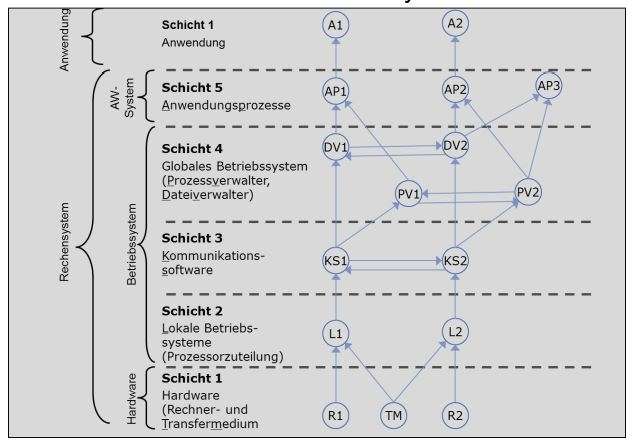
\includegraphics[width=0.4\textwidth]{assets/schichtenmodell.jpg}
					\caption{Schichtenmodell eines Zweirechensystems. Funktionszuordnungen sind nur von unteren auf höhere Schichten möglich.}		
				\end{center}
				\end{figure}	
			\item Binäres Fehlermodell gibt für jede Komponente und das Gesamtsystem an ob sie fehlerfrei sind: $Z: (S \cup \{S\}) \rightarrow \{\texttt{wahr, falsch}\}$. Die Systemfunktion gibt in Abhängigkeit der Komponenten die Funktion des Systems an.
			\item Zuverlässigkeitsblockdiagramm: Zeigt mögliche "`Verbindungspfade"' zwischen den Komponenten, von denen mindestens einer in Takt sein muss. Reihenschaltung von AND-Bausteinen, Parallelschaltung von OR-Bausteinen. Äquivalent zur Systemfunktion.
			\item Negierter Systemfunktionsbaum (alle Blätter werden negiert, alle Verknüpfungen werden vertauscht (\(AND \leftrightarrow OR\))) gibt an, wie sich Fehler des Systems auf Fehler der Komponenten zurückführen lassen.
			\item \textbf{Fehlerbereiche} 
			\begin{itemize}
				\item Komponenten, welche zeitgleich fehlerhaft sein können ohne zu Systemfehlern zu führen. 
				\item Einzelfehlerbereich: Menge von Komponenten, die exakt denselben Fehlerbereichen angehören
				\item Perfektionskern: Das Komplement der Vereinigung aller Fehlerbereiche $\rightarrow$ Komponenten, welche nicht ausfallen dürfen
			\end{itemize}
		\end{itemize}

	\paragraph{Ausfallverhalten}
		\begin{itemize}
			\item Teilausfall: Es fallen nicht alle Funktionen aus
			\item Unterlassungsausfall (Fail-silent-System): Keine Ausgabe fehlerhafter Ergebnisse. Wenn ein Ergebnis ausgegeben wird, ist es korrekt
			\item Anhalteausfall (Fail-stop-System): Keinerlei Ergebnisausgabe mehr
			\item Haftausfall: Komponente gibt ständig denselben Ergebniswert aus
			\item Binärstellenausfall: Ein Fehler verfälscht eine/mehrere Binärstellen
			\item Unkritische Ausfälle (Fail-safe-System)
		\end{itemize}

	\paragraph{Fehlereingrenzung}
		\begin{itemize}
				\item Vertikal: Niedrigere Schichten prüfen Funktionsaufrufe vor Ausführung, Fehlerkorrekturcode in der Hardware, Plausibilitäts-/Konsistenzprüfungen
				\item Horizontal: Isolierung fehlerhafter lokaler Knoten. Problem vor allem bei globalen Schichten.		 
		\end{itemize}
		
	\paragraph{Zuverlässigkeit}
		\begin{itemize}
			\item Um Anforderungen zu erfüllen sind Fehlertoleranz (Redundanz) und Fehlervermeidung wichtig. Zuverlässigkeitskenngrößen können als Verteilungsfunktionen von Lebensdauer, Fehlerbehandlungsdauer und Sicherheit statistisch betrachtet werden:
			\begin{itemize}
				\item $F_L(t)=\frac{N_f(t)}{N}=\frac{N-N_s(t)}{N}=1-R(t)=1-e^{-\lambda t}$ - Wahrscheinlichkeit, dass ein funktionierende System fehlerhaft wird mit Anzahl Komponenten $N$ und $f$ failed oder $s$ survived. Fehlerwarscheinlichkeit exponentialverteilt mit Parameter $\lambda$
				\item $R(t)=\frac{N_s(t)}{N}$ - Überlebenswahrscheinlichkeit
				\item $N_f(t)=N-N_s(t)$
				\item $z(t)=\frac{f_L(t)}{R(t)}$ als Ausfallrate
				\item Ausfallverhalten ("`Badewannenkurve"'): Frühphase (hohe Ausfallwahrscheinlichkeit durch Fertigungsfehler oder defekte Bauteile), Betriebsphase, Spätphase (hohe Ausfallwahrscheinlichkeit durch Verschleiß)
				\item $V=\frac{E(L)}{E(L)+E(B)}$ als Verfügbarkeit mit Lebensdauer $L$ und Behandlungsdauer $B$
				\item $\phi(S)=\sum_{(K_1,\dots,K_n)\in f^{-1}(\texttt{wahr})}\phi(\wedge_{i=1}^n K_i) $ Funktionswahrscheinlichkeit
				\item Weitere Kenngrößen: Gefährdungwahrscheinlichkeit, Sicherheitswahrscheinlichkeit, mittlere Sicherheitsdauer
			\end{itemize}
		\end{itemize}

	\paragraph{Redundanz}
		\begin{itemize}
			\item Statische Redundanz: Vorhandensein redundanter Systeme während des gesamten Einsatzzeitraums (n-von-m-System)
			\item Statische Redundanz/Zuverlässigkeit von n-von-m-Systemen (3-aus-5 vs. 2-aus-3): Das 3-aus-5-System zeigt in der Anfangszeit eine höhere Funktionswahrscheinlichkeit als das 2-aus-3-System. Nach einiger Zeit (Schnittpunkt der beiden Graphen im Bild) kehrt sich dieser Effekt jedoch um. Anfangs sind die einzelnen Funktionswahrscheinlichkeiten noch hoch und bei einem 3-aus-5-System können bis zu 2 Komponenten ausfallen. Wenn die Funktionswahrscheinlichkeit einen bestimmten Punkt unterschreitet, ist ein 2-aus-3-System sicherer, da nur 2 Komponenten zum Betrieb notwendig sind
			\item Dynamische Redundanz: Vorhandensein redundanter Systeme, die erst nach Auftreten eines Fehlers aktiviert werden. Kann zuvor ungenutzt oder fremdgenutzt sein. Auch gegenseitige Redundanz möglich.
		\end{itemize}


\section{Grundlagen der Parallelverarbeitung}
	\paragraph{Formen} 
		\begin{itemize}
			\item Nebenläufigkeit: Objekte werden vollständig gleichzeitig abgearbeitet
			\item Pipelining: Bearbeitung von Objekten wird in sequentielle Teilschritte zerlegt. Pipelinephasen dürfen für verschiedene Objekte überlappen.	
		\end{itemize}

	\paragraph{Ebenen}
		\begin{itemize}
			\item Programmebene: Vom OS organisisert, vollständig unabhängige Einheiten die parallel verarbeitet werden
			\item Prozess/Taskebene: Programm wird in parallel ausführbare Prozesse zerlegt, jeweils eigener Adressraum. Benötigt Synchronisation und Kommunikation, Primitive durch OS implementiert
			\item Blockebene: Threads, teilen sich Adressraum, Synchronisation über Mutex usw., dafür geringerer Aufwand für Erzeugung/ Beendigung/ Wechsel im Vergleich zum Prozess
			\item Anweisungs-/Befehlsebene: Parallele Ausführung elementarer Anweisungen, Optimierende Compiler, Umordnen und Parallelisieren von Befehlen, Superskalar-Technologie
			\item Suboperationsebene: Aufbrechen elementarer Anweisungen in parallel auszuführende Suboperationen durch Compiler, bspw. überlappte Ausführung bei Vektorrechner in Vektorpipeline
		\end{itemize}
		Körnigkeit der Parallelität: Verhältnis Rechenaufwand zu Synchronisationsaufwand.

\section{Klassifikation von Rechnerarchitekturen}
	\paragraph{Flynn'sche Taxonomie} 
		\begin{itemize}
			\item Zahl-, Befehls- und Datenströme
			\item Single Instruction, Single Data (SISD): Uniprozessor
			\item Single Instruction, Multiple Data (SIMD): Vektorrechner, Feldrechner
			\item Multiple Instruction, Single Data (MISD): Zuordnung Umstritten ("`darf es nicht geben"' vs. "`Großrechner oder Supercomputer"')
			\item Multiple Instruction, Multiple Data (MIMD): Multiprozessor
		\end{itemize}
\chapter{Parallelismus auf Machinenbefehlsebene}

\section{Pipelining}
	\begin{itemize}
		\item RISC (Reduced Instruction Set Computers): Einfache, einzyklische Maschinenbefehle; Load/Store-Architektur; Einzyklus-Maschinenbefehle schaffen einheitliches Zeitverhalten, optimierende Compiler
		\item Zerlegung der Ausführung einer Maschinenoperation in Teilphasen, die dann von hintereinander geschalteten Verarbeitungseinheiten taktsynchron ausgeführt werden, wobei jede Einheit genau eine spezielle Teiloperation ausführt. Die Stufen einer Pipeline werden durch Pipeline-Register getrennt
		\item Stufen einer Standard-RISC-Pipeline (DLX-Pipeline): \texttt{Instruction Fetch (IF)}, \texttt{Instruction Decode (ID)}, \texttt{Execution (EX)}, \texttt{Memory Access (MA)} und \texttt{Writeback (WB)}, wobei alle Stufen unterschiedliche Ressourcen benutzen
		\item Idealerweise wird mit jedem Takt ein Befehl beendet, Zykluszeit abhängig von der langsamsten Pipelinestufe
		\item Gleitkommeverarbeitung und Integer-Division: Einführung spezieller Rechenwerke, um die Berechnung innerhalb eines Schrittes ausführen zu können
		\item \textbf{Verfeinerung der Pipeline-Stufen ("`Superpipelining"')}
		\begin{itemize}
			\item Weitere Unterteilung der Pipeline-Stufen
			\item Weniger Logik-Ebenen pro Pipeline-Stufe 
			\item Erhöhung der Taktrate
			\item Führt aber auch zu einer Erhöhung der Ausführungszeit pro Instruktion
		\end{itemize}
		\item Es kann zu Pipeline-Konflikten kommen, die die Instruktionsausführung im nächsten Taktzyklus verhindern. Behebung durch Anhalten der Pipeline bis zur betroffenen Instruktion (Pipeline stall) oder einfügen eines Leerzyklus (Pipeline Bubble). 
		\item \textbf{Konfliktursachen}
		\begin{itemize}
			\item Strukturkonflikte durch gemeinsame Ressourcen
			\item Datenkonflikte aufgrund von Datenabhängigkeiten
			\item Steuerkonflikte bei Instruktionen, die den Befehlszähler (Speicheradresse des auszuführenden Befehls) verändern
		\end{itemize}
	\end{itemize}

\section{Nebenläufigkeit}
	\subsection{Superskalartechnik}
		\begin{itemize}
			\item Mehrfachzuweisung: Pro Takt können mehrere Befehle den Ausführungseinheiten zugeordnet und die gleiche Anzahl von Befehlsausführungen pro Takt beendet werden. Neben Pipelining übliche Parallelisierungsmethode für Mikroprozessoren.
			\item RISC-Eigenschaften bleiben weitestgehend erhalten: Lade-/Speicher-Architektur sowie festes Befehlsformat
			\item Entwurfsziel: Erhöhung des IPC (Instruction per Cycle)
			\begin{itemize}
				\item \textbf{1. In-order-Abschnitt}
				\begin{itemize}
					\item Befehle werden entsprechend ihrer Programmordnung bearbeitet
					\item Umfasst: Befehlsholphase (IF), Dekodierphase (ID) und Zuordnungsphase (Dispatch)
					\item Dynamische Zuordnung der Befehle an die Ausführungseinheiten. Der Scheduler bestimmt die Anzahl der Befehle, die im nächsten Takt zugeordnet werden können
				\end{itemize}
				\item \textbf{Out-of-order-Abschnitt}
				\begin{itemize}
					\item Ausführungsphase
				\end{itemize}
				\item \textbf{2. In-order-Abschnitt}
				\begin{itemize}
					\item Gültigmachen der Ergebnisse entsprechend der ursprünglichen Programmordnung (Retire)
					\item Erhalten der korrekten Programmsemantik (Ausnahmeverarbeitung, Spekulation)
				\end{itemize}
			\end{itemize}
		\end{itemize}

		\par\noindent\rule{\textwidth}{0.4pt}
		\paragraph{FYI: Datenabhängigkeiten}
			\begin{itemize}
				\item Echte Datenabhängigkeiten (Read-after-Write): Ein Operand wurde verändert und kurz darauf gelesen. Da der erste Befehl den Operanden evtl. noch nicht fertiggeschrieben hat (Pipeline-Stufe "`store"' ist weit hinten), würde der zweite Befehl falsche Daten verwenden. Ein "`Shortcut"' im Datenweg der Pipeline kann den Hazard vermeiden. Bei problematischeren Situationen, wenn beispielsweise ein Rechenergebnis zur Adressierung verwendet wird oder bei berechneten und bedingten Sprüngen, ist ein Anhalten der Pipeline aber unumgänglich.
				\item Gegenabhängigkeit (Write-after-Read): Ein Operand wird gelesen und kurz danach überschrieben. Da das Schreiben bereits vor dem Lesen vollendet sein könnte, könnte der Lese-Befehl die neu geschriebenen Werte erhalten. In der normalen Pipeline eher kein Problem.
				\item Ausgabeabhängigkeit (Write-after-Write): Zwei Befehle schreiben auf denselben Operanden. Der zweite könnte vor dem ersten Befehl beendet werden und somit den Operanden mit einem falschen Wert belassen.
			\end{itemize}
		\par\noindent\rule{\textwidth}{0.4pt}

		\paragraph{FYI: Spekulative Ausführung}
			In modernen Prozessoren werden Maschinenbefehle in mehreren Verarbeitungsschritten innerhalb einer Verarbeitungskette (Pipeline) ausgeführt. Um die Leistungsfähigkeit des Prozessors zu maximieren, wird, nachdem ein Befehl in die Pipeline geladen wurde und z. B. im nächsten Schritt mit der Analyse des Befehls fortgefahren werden soll, gleichzeitig mit dem Laden des nächsten Befehles begonnen. Es befinden sich also (meistens) eine ganze Reihe von Befehlen zur sequentiellen Abarbeitung in der Pipeline. Wird jetzt am Ende der Pipeline festgestellt, dass ein bedingter Sprung ausgeführt wird, so sind alle in der Pipeline anstehenden und teilabgearbeiteten Befehle ungültig. Der Prozessor löscht jetzt die Pipeline und lädt diese dann von der neuen Programmcodeadresse neu. Je mehr Stufen die Pipeline hat, desto mehr schon berechnete Zwischenergebnisse müssen verworfen werden und um so mehr Takte wird die Pipeline nur partiell genutzt. Das reduziert die Abarbeitungsgeschwindigkeit von Programmen und reduziert die Energieeffizienz.\footnote{\url{https://de.wikipedia.org/wiki/Sprungvorhersage\#.C3.9Cbersicht}}
			\begin{itemize}
				\item Ziel: Möglichst frühes Erkennen eines Sprungbefehls und Erkennen seiner Sprungzieladresse, damit die Befehle am Sprungziel möglichst ohne NOPs in die Pipeline gegeben werden können
				\item Beinhaltet die Vorhersage, ob ein Sprung ausgeführt wird und berechnet die Zieladresse des Sprungs
				\item \textbf{Statische Sprungvorhersage}
				\begin{itemize}
					\item Vorhersage wird beim Compilieren eingebaut und ändert sich während des Programmablaufs nicht. Genauigkeit etwa bei 55 bis 80 \% (Quelle: Wikipedia)
					\item Geht bei Schleifen davon aus, dass Sprünge häufig ausgeführt werden, während dies bei Auswahlverfahren seltener vorkommt
					\item \textbf{Sprungvorhersagetechniken}
					\begin{itemize}
						\item \texttt{Stall/Freeze}: Wird während der ID-Phase ein Sprungbefehl festgestellt, wird die Pipeline angehalten bis in der EX-Phase bekannt ist, ob der Sprung ausgeführt wird
						\item \texttt{Predict taken}: Geht immer davon aus, dass ein Sprung ausgeführt wird (verwendet bei Schleifen)
						\item \texttt{Predict not taken}: Geht immer davon aus, dass ein Sprung nicht ausgeführt wird (verwendet bei Auswahlverfahren)
					\end{itemize}
				\end{itemize}
				\item \textbf{Dynamische Sprungvorhersage}
				\begin{itemize}
					\item Sprungvorhersage wird zur Laufzeit von der CPU ausgeführt. Genauigkeit bei etwa 98\% (Quelle: Wikipedia)
					\item \textbf{Sprungvorhersagetechniken}
					\begin{itemize}
						\item Der \texttt{Branch History Table} protokolliert die letzten Sprünge in einer Hashtabelle
						\item \texttt{1-Bit-Prädikator}: Zu jedem Sprung wird ein Bit gespeichert. Ist es gesetzt, dann wird ein gespeicherter Sprung genommen. Bei Falschannahme wird dessen Bit invertiert. Problem: Alternierende Sprünge werden nicht berücksichtigt \(\rightarrow\) \texttt{n-Bit-Prädikator}
						\item \texttt{2-Bit-Prädikator}: Speichert vier Zustände und setzt das Korrektheitsbit erst nach \texttt{2} Fehlschlägen neu. Zustände sind \texttt{Predict strongly taken (11)}, \texttt{Predict weakly taken (10)}, \texttt{Predict weakly not taken (01)} und \texttt{Predict stronly not taken (00)}. In der Praxis bringen Prädikatoren mit mehr als 2 Bit kaum Vorteile.
					\end{itemize}
					\item \textbf{Sprungzielvorhersagetechniken}
					\begin{itemize}
						\item Erweitert die Sprungvorhersage um eine Sprungzielvorhersage. Somit kann der Programmzähler sofort auf dieses Sprungziel gesetzt werden und die dortigen Instruktionen können in die Pipeline laden werden
						\item Sprungzielcache: \texttt{Branch Target Address Cache} (Tabelle: Adresse der Verzweigung \(\rightarrow\) Sprungzieladresse) und \texttt{Branch Target Buffer} (Direct-mapped-Cache) speichern die Adresse der Verzweigung und das entsprechende Sprungziel
						\item \texttt{Branch Prediction Buffer}: Paralleler Zugriff auf den Befehlsspeicher und den BPB in der Befehlsholphase. Falls die Instruktion eine Verzweigung ist, bestimmt die Vorhersage die nächste zu holende Instruktion und berechnet die Adresse des Befehls. Nach Ausführung der Verzweigung wird die Sprungsvorhersage verifiziert und der Eintrag im BPB ggf. aktualisiert
					\end{itemize}
				\end{itemize}
			\end{itemize}
		\par\noindent\rule{\textwidth}{0.4pt}

		\paragraph{Superskalare Prozessorpipeline}
			\begin{itemize}
				\item \textbf{Befehlsholphase (IF-Phase)}
				\begin{itemize}
					\item \textbf{Befehlsbereitstellung}
					\begin{itemize}
						\item Holen mehrerer Befehle aus dem Befehlscache in der Befehlsholpuffer (Anzahl entspricht typischerweise der Zuordnungsbreite)
						\item Welche Befehle geholt werden hängt von der Sprungvorhersage ab
					\end{itemize}
					\item \textbf{Verzweigungseinheit}
					\begin{itemize}
						\item Überwacht die Ausführung von Sprungbefehlen
						\item Spekulatives Holen von Befehlen und Spekulation über den weiteren Programmverlauf (Verwendung hierzu der Vorgeschichte)
						\item Gewährleistet im Falle einer Fehlspekulation die Abänderung der Tabellen sowie das Rückholen der fälschlicherweise ausgeführten Befehle
					\end{itemize}
					\item \textbf{Sprungvorhersage} 
					\begin{itemize}
						\item Statisch: Vorhersagerichtung für einen Befehl immer gleich. Für superskalare Prozessorarchitekturen zu unflexibel
						\item Dynamisch: Verzweigungsrichtung in Abh. der Vorgeschichte, berücksichtigt Programmberhalten. Dafür hoher Hardwareaufwand. Lernen durch Abgleich mit Realität und Ändern zukünftiger Voraussagen. Mit zwei Bits feingranularer möglich.
					\end{itemize}
					\item Befehlsholpuffer: Entkoppelt die IF-Phase von der ID-Phase
				\end{itemize}
				\item \textbf{Dekodierphase (ID-Phase)}
				\begin{itemize}
					\item Dekodierung der im Befehlspuffer abgelegten Befehle. Die Anzahl entspricht typischerweise der Befehlsbereitstellungsbandbreite
					\item Bei CISC-Architekturen (z.B. IA-32): Mehrere Schritte zur Dokodierung notwendig. Bestimmung der Grenzen der geholten Befehle sowie Generierung einer Folge von RISC-ähnlichen Befehlen. Ermöglicht effizientes Pipelining und superskalare Verarbeitung
					\item Registerumbenennung: Dynamische Umbenennung der Operanden- und Resultatsregister. Zur Laufzeit wird für jeden Befehl das jeweils spezifizierte Zielregister auf ein unbelegtes physikalisches Register abgebildet. Automatische Auflösung von Namensabhängigkeitskonflikten (Write-after-Read, Write-after-Write, Read-after-Write)
					\item Befehlsfenster (instruction window): Durch das Schreiben der Befehle in ein Befehlsfenster sind diese durch die Sprungvorhersage frei von Steuerflussabhängigkeiten und aufgrund der Registerumbenennung frei von Namensabhängigkeiten
				\end{itemize}
				\item \textbf{Zuordnungsphase (Dispatch)}
				\begin{itemize}
					\item Zuführung der im Befehlsfenster wartenden Befehle zu den Ausführungseinheiten sowie dynamischer Auflösung von echten Datenabhängigkeiten (Befehle die den Output eines anderen Befehls benötigen) und Ressourcenkonflikten
					\item Zuordnung bis zur maximalen Zuordnungsbandbreite pro Takt
					\item Zweistufige Zuweisung: Jeder Ausführungseinheit ist ein Umordnungspuffer (den sie sich ggf. mit anderen Ausführungseinheiten teilt) vorgelagert. Zuordnung eines Befehls an einen Umordnungspruffer kann nur erfolgen, wenn dieser einen freien Platz hat, ansonsten müssen die nachfolgenden Befehle warten (Auflösung von Ressourcenkonflikten)
					\item Rückordnungspuffer (Reorder buffer): Festhalten der ursprünglichen Befehlsanordnung sowie Protokollierung der Ausführungszustände der Befehle in den folgenden Phasen
				\end{itemize}
				\item \textbf{Befehlsausführung}
				\begin{itemize}
					\item Ausführung der im Opcode spezifizierten Operation und Speichern des Ergebnisses im Zielregister (Umbenennungsregister)
					\item Completion: Eine Instruktion beendet ihre Ausführung, unabhängig von der Programmordnung, wenn das Ergebnis bereitsteht. Danach: Bereinigung der Reservierungstabellen und Aktualisieren des Rückordnungspuffer
				\end{itemize}
				\item \textbf{Rückordnungsstufe (Retire)}
				\begin{itemize}
					\item Commitment: Nach Vervollständigung beenden die Befehle ihr Bearbeitung (Commitment) und werden in der Programmreihenfolge gültig gemacht. Ggf. werden Ergebnisse aus Umbenennungsregistern gültig gemacht durch zurückschreiben. 
					\item \textbf{Bedingungen für Commitment}
					\begin{itemize}
						\item Die Befehlsausführung ist vollständig
						\item Alle Befehle, die in der Programmordnung vor dem Befehl stehen, haben bereits ihre Bearbeitung beendet oder beenden diese im selben Takt
						\item Der Befehl hängt von keiner Spekulation ab
						\item Vor oder während der Bearbeitung ist keine Unterbrechung aufgetreten
					\end{itemize}
					\item \textbf{Precise interrups}
					\begin{itemize}
						\item Alle Resultate, die in der Programmausführung vor dem Befehl stehen, werden gültig gemacht; die Ergebnisse aller nachfolgenden werden verworfen
						\item Das Ergebnis des Befehls, der die Unterbrechung verursacht hat, wird in Abhängigkeit der Unterbrechung und der Architektur gültig gemacht oder verworfen
						\item Komplexe Hardware notwendig
					\end{itemize}
				\end{itemize}
			\end{itemize}

		\paragraph{Dynamische Methoden zur Erkennung und Auflösung von Datenkonflikten am Beispiel Tomasulo (IBM 360/91)}
			\begin{itemize}
				\item Ziel: Fortsetzung der Ausführung von Befehlen, auch wenn Datenabhängigkeiten vorliegen
				\item \textbf{Vorgehen zum Verhindern von Konflikten}
				\begin{itemize}
					\item Read-after-Write: Der Prozessor verfolgt, wann Operanden zur Verfügung stehen
					\item Write-after-Read und Write-after-Write: Nutzung von \textit{Reservierungstabelle/Reservation Stations}, die Registerinhalte zwischenspeichert und so vor vorzeitigem Überschreiben schützt
				\end{itemize}
				\item \textbf{Funktionsweise\footnote{\url{https://de.wikipedia.org/wiki/Tomasulo-Algorithmus\#Funktionsweise}}}
				\begin{itemize}
					\item Issue: Der Befehl an der aktuellen Position in der Operation Queue wird dekodiert und entsprechend seiner auszuführenden Operation in eine passende Reservation Station eingetragen. Operanden werden direkt aus der Registerdatei übernommen, wenn sie gültig sind. Dieser Vorgang wird als Registerumbenennung bezeichnet. Steht ein Operand noch nicht zur Verfügung, wird stattdessen die Adresse der RS eingetragen, die den Wert gerade berechnet. Ist keine passende RS frei, verbleibt der Befeht in der Operation Queue und die Zuweisung wird im nächsten Takt erneut versucht
					\item Execute: Sobald alle Operanden in der Reservation Station zur Verfügung stehen, wird die Operation an die FU weiter gegeben und ausgeführt. Andernfalls wird der Common Data Bus/Ergebnisbusses auf eingehende Werte beobachtet und fehlende Operanden übernommen, wenn die Adresse der Quell-RS mit der benötigten Adresse übereinstimmt
					\item Write Result: Sobald das Ergebnis der Operation berechnet wurde, wird es mitsamt der Adresse der ausgeführten RS auf den Common Data Bus gelegt und somit für die RS sichtbar, welche auf das Ergebnis warten
				\end{itemize}
			\end{itemize}

		\paragraph{Zusammenfassung Superskalartechnik}
			\begin{itemize}
				\item Aus einem sequentiellen Befehlsstrom werden Befehle zur Ausführung angestoßen
				\item Die Zuordnung erfolgt dynamisch durch die Hardware
				\item Es kann mehr als ein Befehl zugewiesen werden. Die Anzahl der zugewiesenen Befehle pro Takt wird dynamisch von der Hardware bestimmt und liegt zwischen Null und der maximalen Zuordnungsbreite
				\item Komplexe Hardwarelogik für dynamische Zuweisung notwendig
				\item Mehrere, voneinander unabhängige Funktionsanweisungen verfügbar
				\item Mikroarchitektur, da der Befehlssatz nicht verändert wird. Technisch gesehen "`nur"' eine Erweiterung der Pipeline
				\item \textbf{FYI: Formen}\footnote{\url{https://de.wikipedia.org/wiki/Superskalarit\%C3\%A4t}}
				\begin{itemize}
					\item Superskalare Prozessoren mit statischem Scheduling: Die Anzahl der pro CPU-Zyklus parallel ausführbaren Befehle ist nicht vorgegeben, sondern wird durch die CPU dynamisch bestimmt. Da es sich um statisches Scheduling handelt, wird die Reihenfolge der Befehle vom Compiler vorgegeben
					\item Superskalare Prozessoren mit dynamischem Scheduling: Die CPU bestimmt sowohl, welche Befehle parallel ausgeführt werden, als auch die Reihenfolge, in der dies geschieht (Out-of-order execution)
					\item VLIW-Prozessoren: Die Architekturen benutzen deutlich längere Befehle, in denen die parallel auszuführenden Befehle vorgegeben werden
				\end{itemize}
			\end{itemize}

	\subsection{Very Long Instruction Word (VLIW)}
		\begin{itemize}
			\item Ziel: Beschleunigen der Abarbeitung durch Parallelität auf Befehlsebene
			\item Breites Befehlsformat, das in mehrere Felder aufgeteilt ist, aus denen die Funktionseinheiten (EX) gesteuert werden
			\item Eine VLIW-Architektur mit \texttt{n} unabhängigen Funktionseinheiten kann bis zu \texttt{n} Operationen gleichzeitig ausführen
			\item Operationen ähnlich zu Befehlssätzen in RISC-Architektur
			\item Steuerung der parallelen Abarbeitung zur Übersetzungszeit (automatisch parallelisierender Compiler). Der Compiler gruppiert die Befehle, die parallel ausgeführt werden können
			\item Die Gruppengröße ist abhängig von der Anzahl der Ausführungseinheiten
			\item Vorteil gegenüber superskalaren Prozessoren: Weniger Hardware-Logik notwendig \(\rightarrow\) mehr Platz auf dem Chip für zusätzliche Funktionalität bei beispielsweise mehr Ausführungseinheiten
			\item Vorteile: Einfacher Kontrollpfad sowie Ausnutzungsmöglichkeiten der Compilertechnik (z.B. Softwarepipeling, Schleifenparallelisierung, etc.)
			\item Nachteil: Portierung des Codes auf andere Prozessoren eventuell schwierig
		\end{itemize}

		\paragraph{Statische Steuerung der parallelen Abarbeitung}
			\begin{itemize}
				\item Zusätzliche Aufgaben für den Compiler: Code-Generierung (Kontrollflussanalyse, Datenflussanalyse, Datenabhängigkeitsanalyse), Schleifenparallelisierung, Scheduling (Beispiel auf Folie 8-33)
				\item Software-Pipelining: Technik zur Reorganisation von Schleifen. Jede Iteration im generierten Code enthält Befehle aus verschiedenen Iterationen der ursprünglichen Stufe
			\end{itemize}

	\subsection{Multithreading (Mehrfädigkeit)}
		\begin{itemize}
			\item Entwurfsziel: Reduzieren der Untätigkeits- oder Latanzzeiten, die bei Speicherzugriffen (insbesondere Cache-Fehlzugriffe) entstehen
			\item Ziel: Parallele Ausführung mehrerer Kontrollfäden
			\item \textbf{Ansätze}
			\begin{itemize}
				\item Interleaved Multithreading (cycle-by-cycle): In jedem Zyklus wird ein Befehl aus einem anderen Kontrollfaden geholt und ausgeführt. Problem: Wenn Thread ohne Wartezeiten ausgeführt werden könnte, ist er mit dieser Technik deutlich langsamer
				\item Blocked Multithreading: Die Befehle eines Threads werden solange ausgeführt bis ein Ereignis eintritt, das eine lange Wartezeit nach sich zieht. Bearbeitung daher nicht so stark verlangsamt, die Pipeline muss jedoch bei Wechsel geleert und neugestartet werden, das ist nur bei langen Wartezeiten sinnvoll
				\item Simultaneous Multithreading: Mehrfach superskalar, die Ausführungseinheiten werden über eine Zuordnungseinheit aus mehreren Befehlspuffern versorgt. Jeder Befehlspuffer stellt einen anderen Befehlsstrom dar und hat einen eigenen Registersatz zugeordnet. Trade-off zwischen Geschwindigkeit pro Thread und Durchsatz an Threads.
			\end{itemize}
		\end{itemize}


\chapter{Multiprozessoren - Parallelismus auf Prozess-/Blockebene}

\section{Allgemeine Grundlagen}
	\paragraph{Parallele Architekturmodelle}
		\begin{itemize}
			\item \textbf{Multiprozessor mit gemeinsamem Speicher: Uniform Memory Access (UMA)}
			\begin{itemize}
				\item Gleichberechtigter Zugriff der Prozessoren auf die Betriebsmittel
				\item Gemeinsamer Speicher mit globalem Adressraum, Austausch von Daten über gemeinsamen Speicher durch LS-Operationen
				\item Beispiele: Symmetrischer Multiprozessor (SMP), Multicore-Prozessor
			\end{itemize}
			\item \textbf{Multiprozessor mit verteiltem Speicher: No Remote Memory Access (NORMA)}
			\begin{itemize}
				\item Physikalisch verteilter Speicher
				\item Jeder Knoten mit einem privaten Adressraum
				\item Kommunikation durch Nachrichtenaustausch über ein Interconnect Network
				\item Beispiel: Cluster
			\end{itemize}
			\item \textbf{Multiprozessor mit verteiltem gemeinsamen Speicher: Non-Uniform Memory Access (NUMA)}
			\begin{itemize}
				\item Globaler Adressraum über mehreren, exklusiv jeweils einem Prozessor zugeordneten Speichereinheiten
				\item Speicher physikalisch verteilt
				\item Zugriff auf entfernten Speicher über LS-Operationen (über ein Interconnect Network)
				\item Beispiel: Cache-Coherent Non-Uniform Memory Access oder Distributed shared Memory (DSM)
			\end{itemize}
		\end{itemize}

\section{Parallele Programmiermodelle}
	Programmiermodell: Abstraktion einer parallelen Maschine, die spezifiziert, wie Teile des Programms parallel abgearbeitet werden und wie Informationen ausgetauscht werden können

	\begin{itemize}
		\item Aufteilung der Arbeit (work partitioning): Identifizieren der Teilaufgaben, die parallel ausgeführt und auf mehrere Prozessoren verteilt werden können (Programmsegmente müssen unabhängig von einander sein)
		\item Koordination (coordination): Koordination/Synchronisierung/Kommunikation (zwischen) den/der Prozesse
		\item Sychronisation und Koordination: Austausch von Informationen über gemeinsamen Speicher oder über explizite Nachrichten. Zusätzlicher Zeitaufwand hat Auswirkung auf die Ausführungszeit des parallelen Programms
		\item: Parallelismus: Daten (z.B. Matrixmultiplikation) oder Funktion (unabhängige Funktionen) 
		\item \textbf{Gemeinsamer Speicher (Shared Memory)}
		\begin{itemize}
			\item Verwendung konventioneller Speicheroperationen für die Kommunikation über gemeinsame Adressen
			\item Atomare Synchronisationsoperationen
		\end{itemize}
		\item \textbf{Nachrichten (Message Passing)}
		\begin{itemize}
			\item Kein gemeinsamer Adressbereich, Kommunikation der Prozesse (Threads) mit Hilfe von Nachrichten
			\item Kommunikationsarchitektur: Verwendung von korrespondierenden Send- und Receive-Operationen
		\end{itemize}
		\item Beispiel: OpenMP für gemeinsamen Speicher, MPI für verteilten Speicher
	\end{itemize}
	Durchzuführende Schritte beim Parallelisierungsprozess: Dekomposition, Zuweisung, Festlegung, Abbildung


\section{Quantitative Maßzahlen}
	\paragraph{Definitionen}
		\begin{itemize}
			\item \(P(1)\) bzw. \(P(n)\): Anzahl der auszuführenden Operationen/Tasks auf einem Einprozessor- bzw. Multiprozessorsystem
			\item \(T(1)\) bzw. \(T(n)\): Ausführungszeit auf einem Einprozessor- bzw. Multiprozessorsystem in Schritten oder Takten
		\end{itemize}

	\paragraph{Parallelitätsprofil}
		\begin{itemize}
			\item Misst die entstehende Parallelität in einem Programm oder bei der Ausführung auf einem Parallelrechner und liefert so eine Vorstellung von der inhärenten Parallelität eines Algorithmus/Programms
			\item Grafische Darstellung: XY-Diagramm mit Anzahl der parallelen Aktivitäten in zeitlicher Abhängigkeit \(\rightarrow\) Perioden von Berechnungs- Kommunikations- und Untätigkeitszeiten sind erkennbar
			\item Der Parallelitätsgrad \(PG(t)\) gibt die Anzahl der Tasks an, die zu einem Zeitpunkt parallel bearbeitet werden können
			\item Leistungsangaben zu Multiprozessorsystemen werden mit Leistungsangaben zu Einprozessorsystemen in Beziehung gesetzt
			\item \textbf{Parallelindex I (Mittlerer Grad des Parallelismus)}
			\begin{itemize}
				\item Durchschnittliche Parallelität pro Zeiteinheit
				\item Kontinuierlich: \(I = \frac{1}{t_2-t_1}\int_{t_1}^{t_2}PG(t)dt\)
				\item Diskret: \(\Big(\sum_{i=1}^m i\cdot t_i\Big)~/~\Big(\sum_{t=1}^mt_i\Big)\)
			\end{itemize}
			\item $S(n)=\dfrac{T(1)}{T(n)}$ gibt den Speedup an, die Effizienz berechnet sich zu $E(n)=\dfrac{S(n)}{n}$
			\item $U(n)=\dfrac{I(n)}{n}$ als Auslastung 
		\end{itemize}

	\paragraph{Skalierbarkeit eines Parallelrechners}
		\begin{itemize}
			\item Das Hinzufügen von weiteren Verarbeitungselementen führt zu einer kürzeren Gesamtausführungszeit, ohne dass das Programm geändert werden muss
			\item Bei fester Problemgröße und steigender Prozessorzahl wird eine Sättigung eintreten
		\end{itemize}

	\paragraph{Gesetz von Amdahl}
		\begin{itemize}
			\item Ein Programm kann nie vollständig parallel ausgeführt werden, da einige Teile wie Prozess-Initialisierung oder Speicherverwaltung nur einmalig auf einem Prozessor ablaufen oder der Ablauf von bestimmten Ergebnissen abhängig ist\(\rightarrow\) Zerlegung des Programmlaufs in Abschnitte, die entweder vollständig sequentiell oder vollständig parallel ablaufen und fasst sie zu jeweils einer Gruppe zusammen\footnote{\url{https://de.wikipedia.org/wiki/Amdahlsches_Gesetz\#Beschreibung}}
			\item Gesamtausführungzeit (Gesetz von Amdahl): \(T(n) = T(1) \cdot \frac{1-a}{n} + T(1) \cdot a\), \(a\): Anteil des Programms, der nur sequentiell ausgeführt werden kann
			\item Superlinearen Speedup kann es nicht geben, da jeder paralle Algorithmus einen sequentiellen Teil hat, der die Beschleunigung begrenzt: \(1 \le S(n) \le n\). Tritt jedoch in der Realität dennocg auf: Ursache ist beispielsweise, dass bei einem Mehrprozessorsystem die Daten vollständig in lokale Caches und Hauptspeicher passen (kein Verlust durch häufige Seitenwechsel)
		\end{itemize}


\section{Verbindungsnetzwerke}
	\begin{itemize}
		\item \textbf{Verbindungsnetzwerke in Multiprozessoren}
		\begin{itemize}
			\item Ermöglichen die Kommunikation und Kooperation zwischen den Verarbeitungselementen
			\item Einsatz: Chip-Multiprozessor (NoC, beispielsweise Verbinden des gemeinsamen L2-Cache), Multiprozessor mit gemeinsamem oder verteilten Speicher
		\end{itemize}
		\item \textbf{Charakterisierung von Verbindungsnetzwerken}
		\begin{itemize}
			\item \textbf{Latenz}
			\begin{itemize}
				\item Übertragungszeit einer Nachricht \(T_{msg}=t_{\text{message startup time}}+t_{\text{message transfer time}}\), Vorraussetzung: Das Netzwerk ist konfliktfrei
				\item Kanalverzögerung (channel delay): Dauer für die Belegung eines Kommunikationskanals durch eine Nachricht
				\item Schaltverzögerung: Zeit, die benötigt wird um einen Weg zwischen zwei Knoten aufzubauen. Pfadberechnung oder Wegfindung
				\item Blockierungszeit: Wird verursacht, wenn zu einem Zeitpunkt mehr als eine Nachricht auf eine Netzwerkressource zugreifen will
			\end{itemize}
			\item Durchsatz/Übertragungsbandbreite
			\item Bisektionsbandbreite: Maximale Bandbreite, die das Netzwerk über die Bisektionslinie (teilt das Netzwerk in zwei Hälften) transportiert werden kann
			\item Diameter/Durchmesser: Maximale Distanz zwischen zwei Prozessoren/Knoten
			\item Verbindungsgrad: Anzahl der Direktverbindungen pro Knoten
			\item Mittlere Distanz: Durchschnittlicher Abstand zwischen zwei Knoten
			\item Komplexität/Erweiterbarkeit/Skalierbarkeit
			\item Ausfalltoleranz/Redundanz
			\item \textbf{Art des Transfers}
			\begin{itemize}
				\item Durchschalte- oder Leistungsvermittlung: Schalten einer Direktverbindung zwischen zwei Knoten, blockierungsfrei, kurze Latenz, gut geeignet für lange Nachrichten
				\item Paketvermittlung: Datenpakete fester Länge werden entsprechend einem Wegfindealgorithmus übertragen, geeignet für kurze Nachrichten
			\end{itemize}
		\end{itemize}
		\item \textbf{Verbindungsnetzwerk (IN)}
		\begin{itemize}
			\item Knoten: über Netzwerkschnittstelle verbunden
			\item Switch/Schaltelement: setzt Verbindungen
			\item Link: Verbindungen, synchron mit gemeinsamer Taktquelle oder asynchron über Handshake
			\item Nachricht: Uni-/Multi-/Broadcast, Fixed length möglich
		\end{itemize}
		\item \textbf{Datentransfer}
		\begin{itemize}
			\item Durchschalte- oder Leistungsvermittlung/Circuit Switching: Es wird eine direkte Verbindung zwischen Knoten geschaltet, keine Unterbrechung, keine Routing-Information im Paket nötig. Dafür blockieren der Leitung
			\item Paketvermittlung/Packet switching: Pakete mit fester Länge werden geroutet, bedarfsorientiertes Blocken der Leitungen. Store and forward von Paketen oder Cut-through Switching
		\end{itemize}
		\item End-to-end packet latency model: Betrachte Gesamtlatenz. $\texttt{E2E latency}=\texttt{Sender Overhead +  \texttt{Time of flight}+\texttt{Transmission time}+\texttt{Routing time}+\texttt{Receiver Overhead}}$
		\item Effektive Bandbreite: $EB=\dfrac{\texttt{Paketgröße}}{max{\texttt{Sender OH}, \texttt{Empfänger OH}, \texttt{Übertragungszeit}}}$
		\item \textbf{Verbindungsnetze}
		\begin{itemize}
			\item \textbf{Statische Verbindungsnetze}
			\begin{itemize}
				\item Nach Aufbau des Verbindungsnetzes bleiben die Strukturen fest
				\item Vorhersagbare Kommunikationsmuster zwischen Knoten
				\item Vollständige Verbindung: Alle Knoten sind miteinander verbunden. Höchste Leistungsfähigkeit aber nicht praktikabel bei hoher Prozessorzahl (Aufwand steigt qudratisch mit der Prozessorzahl)
				\item Gitterstrukturen: Verbinden benachbarte Knoten. Disjunkte Bereiche können parallel genutzt werden, allerdings oft mehrere Schritte notwendig (bei unbenachbarten Knoten)
				\item Unidirektionaler Ring: Nachrichten werden vom Quellknoten zum Zielknoten geschickt. Bei Ausfall bricht die Kommunikation zusammen
				\item Bidirektionaler Ring: Übertragung kann die kürzeren der beiden Wege wählen. Bei einer Unterbrechung bleibt die Kommunikation bestehen
				\item Chordaler Ring: Hinzufügen weiterer Direktverbindungen zur Erhöhung der Fehlertoleranz
				\item Baumstruktur: Teilweise mit steigender Anzahl an Kommunikationskanälen in Richtung Wurzel
				\item Diverse Kubusstrukturen, beispielsweise Hyperkubus: Binäre Bezeichnung der Knoten ermöglicht Routenbestimmung (benachbarte Knoten unterscheiden sich um genau eine Stelle, Start- und Zieladresse werden per XOR verknüpft). Allerdings schlechte Skalierbarkeit, da bei jeder Erweiterung der Knotengrad steigt und alle Knoten erweitert werden müssen
				\begin{itemize}
					\item Anzahl der Knoten eines \(K\)-nären \(n\)-Kubus: \(N = K^n\)
					\item Knoten-/Verbindungsgrad: \(2n\)
				\end{itemize}
			\end{itemize}
			\item \textbf{Dynamische Verbindungsnetze}
			\begin{itemize}
				\item Geeignet für dynamische Anwendungen mit variablen und nicht regulären Kommunikationsmustern
				\item Bus: Wird von allen an den Bus angeschlossenen Prozessoren gemeinsam genutzt. Verwendung von Cache-Speichern (mit Cache-Kohärenz-Protokollen zur Synchronisiation) zur Reduzierung des Busverkehrs. Synchronisation durch Split-Phase Busprotokollen erforderlich
				\item Kreuzschienenverteiler (Crossbar)
				\begin{itemize}
					\item Hardwaresystem, das in einer Menge an Prozessoren zwischen allen disjunkten Paaren von Prozessoren blockierungsfreie Direktverbindungen zur Kommunikation aufbauen kann. Schaltelemente an allen Kreuzungspunkten \(\rightarrow\) hoher Hardwareaufwand
					\item Schalterelemente (2x2-Kreuzschienenverteiler) bestehen aus Zweierschaltern mit je zwei Ein- und Ausgängen, die entweder durch- oder über kreuz schalten können
				\end{itemize}
				\item Omega-Netz: Besteht aus \(\frac{N\cdot log_k(N)}{k}\) Crossbars bei \(N\) Knoten mit Switch-Grad \(k\). Nicht blockierungsfrei
				\item Mischpermutationnetz: Kreisverschiebung der Adressbits
				\item Allgemeine Beispiele für dynamische Verbindungsnetzwerke: Bus, Kreuzschiene, Schaltnetzwerk
				\item Kreuzpermutation: Abbildung auf invertierte ID. Beispielsweise \(001 \longrightarrow 100\)
				\item Mischpermutation: Addieren von \(\forall 0..\frac{n-1}{2}:2n\). Beispielsweise \(000 \longrightarrow 000, 001 \longrightarrow 010\). Die obere Hälfte invertiert
			\end{itemize}
		\end{itemize}
	\end{itemize}


\section{Multiprozessoren mit gemeinsamem Speicher}
	\begin{itemize}
		\item Gültigkeitsproblem: Paralleler Zugriff mehrere Prozessoren auf den Hauptspeicher \(\rightarrow\) mehrere Kopien des gleichen Speicherwortes müssen miteinander in Einklang gebracht werden
		\item Inklusionseigenschaft bei Caches: Der Inhalt des Caches auf der höchsten Stufe ist auch in den Caches niedrigerer Stufen enthalten
	\end{itemize}	
	\paragraph{Cache-Kohärenz-Problem}
		\begin{itemize}
			\item \textbf{1. Fall (IO-Problem)} System mit einem Mikroprozessor und weiteren Komponenten mit Master-Funktion (ohne Cache)
			\begin{itemize}
				\item Zusätzlicher Master (beispielsweise DMA-Controller) kann Kontrolle über den Bus übernehmen und prozessorunabhängig auf den Hauptspeicher zugreifen
				\item Problem: Prozessor oder DMA-Controller lesen eventuell veraltete Daten (stale data)
				\item \textbf{Lösungen des Kohärenzproblems}
				\begin{itemize}
					\item Non-Cacheable Data: Der gemeinsam genutzte Speicherbereich wird nicht gecacht bzw. mit "`non-cacheable gekennzeichnet"'
					\item Cache-Clear/Cache-Flush: Nach einem DMA-Vorgang wird der Cache automatisch neu geladen
				\end{itemize}
			\end{itemize}
			\item \textbf{2. Fall: Speichergekoppeltes Multiprozessorsystem}
			\begin{itemize}
				\item Mehrere Prozessoren mit jeweils eigenem Cache-Speicher sind über einen Systembus an einen gemeinsamen Hauptspeicher angebunden
			\end{itemize}
		\end{itemize}

	\paragraph{Kohärenz}
		\begin{itemize}
			\item Vereinfachte Definition "`Cache-Kohärenz"': Ein Speichersystem ist kohärent, wenn jeder Lesezugriff auf ein Datum den aktuellen, geschriebenen Wert dieses Datums liefert
			\item Ein paralleles Programm, das auf einem Multiprozessor läuft, kann mehrere Kopien eines Datums in mehreren Caches haben
			\item \textbf{Möglichkeiten, die Kohärenzanforderungen zu erfüllen}
			\begin{itemize}
				\item Write-invalidate-Protokoll: Sicherstellen, dass ein Prozessor exklusiven Zugriff auf ein Datum hat, bevor er schreiben darf. Vor dem Verändern einer Kopie in einem Cache-Speicher müssen alle Kopien in anderen Cache-Speichern für ungültig erklärt werden
				\item Write-update-Protokoll: Beim Verändern einer Kopie in einem Cache-Speicher müssen alle Kopien in anderen Cache-Speichern ebenfalls verändert werden, wobei die Aktualisierung auch verzögert (allerdings spätestens beim Zugriff) erfolgen kann
			\end{itemize}
		\end{itemize}

	\paragraph{Kohärenzprotokolle}
		\begin{itemize}
			\item Bus-Snooping: Caches sind an einem gemeinsamen Bus und beobachten diesen, um feststellen zu können, ob sie eine Kopie eines Blocks enthalten, der benötigt wird
			\item MESI-Kohärenzprotokoll (Hardware)
			\begin{itemize}
				\item Jeder Cache verfügt über Snoop-Logik und Steuersignale: Invalidate-Signal (zum Invalidieren von Einträgen in anderen Caches), Shared-Signal (zeigt an, ob ein zu ladender Block bereits als Kopie besteht) und Retry-Signal (Aufforderung für den Prozessor das Laden eines Blocks abzubrechen. Nachdem ein anderer Prozessor aus dem Cache in den Hauptspeicher zurückgeschrieben hat wird das Laden wieder aufgenommen)
				\item Erweiterung jeder Cache-Zeile um zwei Steuerbits zum Anzeigen der Zustände
				\begin{itemize}
					\item Invalid (I): Die Cache-Zeile ist ungültig. Mittels Shared-Signal zeigen die anderen Steuerungen an, ob sie diesen Block gespeichert haben (shared read hit/miss). Davon abhängig erfolgt der Übergang in \(S\) oder \(E\). Bei einem Write-Miss erfolgt der Übergang in \(M\)
					\item Shared (S): Der Speicherblock existiert sowohl lokal als auch in anderen Caches. Bei einem Schreibzugriff übergang in Zustand \(M\) und Ausgeben des Invalidate-Signals
					\item Exclusive (E): Der Speicherblock existiert exklusiv nur in der Zeile dieses Caches. Lese- und Schreibzugriffe möglich, ohne den Bus benutzen zu müssen. Nach Schreibzugriff, Wechsel in \(E\)
					\item Modified (M): Der Speicherblock existiert nur lokal und ist nach dem Laden verändert worden. Bei einem externen Zugriff durch einen anderen Prozessor muss dieser in den Hauptspeicher zurückkopiert werden. Der externe Prozessor wird über das Retry-Signal informiert, dass zunächst zurückgeschrieben werden muss
				\end{itemize}
				\item Zustandsgraphen und Beispiel in den Folien\footnote{VL-07 Folie 2-40 bis 2-47}
			\end{itemize}
			\item MOESI-Kohärenzprotokoll: Erweitert das MESI-Protokoll um den zusätzlichen Zustand \texttt{Owned} (\texttt{O}). Es vermeidet das Zurückschreiben von modifizierten Cache-Lines, wenn andere CPUs diese lesen wollen. Stattdessen wird der aktuelle Wert bei jeder Veränderung zwischen den Caches direkt propagiert\footnote{\url{https://de.wikipedia.org/wiki/MOESI}} (praktisch, wenn ein Prozessor einen Wert in seinen Cache läd, der bereits in einem anderen Cache existiert)
			\item \textbf{Distributed Shared Memory}
			\begin{itemize}
				\item Multiprozessor mit verteiltem, gemeinsamem Speicher ohne Möglichkeit, die Broadcasteigenschaft des Busses zu nutzen
				\item Verzeichnisbasierte, tabellenartige Cache-Kohärenzprotokolle, die in Hardware oder Software implementiert sein können
				\item Die Tabelle protokolliert für jeden Block im loken Speicher, ob dieser in den lokalen oder einen entfernten Cache-Speicher übertragen worden ist und hält die Zustände als Kopien
				\item Zustände werden ähnlich denen des MESI-Protokolls definiert
			\end{itemize}
		\end{itemize}

	\paragraph{Speicherkonsistenz}
		\begin{itemize}
			\item Sequentielle Konsistenz: Ein Multiprozessorsystem heißt sequentiell konsistent, wenn das Ergebnis einer beliebigen Berechnung dasselbe ist, als wenn die Operation sequentiell auf einem Einprozessorsystem ausgeführt worden ist
			\item Atomar Schreibzugriffe
			\item Programmierer geht von sequentieller Konsistenz aus \(\rightarrow\) sehr starke Leistungseinbußen bzgl. der Implementierung und der Leistung. Verbietet vorgezogene Ladeoperationen und nicht-blockierende Caches
			\item Schwache Konsistenz (Speicherkonsistenzmodell)
			\begin{itemize}
				\item Konkurrierende Zugriffe auf gemeinsame Daten werden durch Sychronisationen geschützt (beispielsweise Semaphoren oder Mutecies)
				\item Idee: Konsistenz des Speicherzugriffs wird nicht mehr zu allen Zeiten gewährleistet sondern nur zu definierten Synchronisationspunkten. Einführung "`kritischer Bereiche"' innerhalb denen keine Synchronisation gewährleistet sein muss
				\item Voraussetzung: Hardware oder softwareseitige Unterscheidung der Synchronisationsbefehlen von den LS-Befehlen und eine sequentiell konsistente Implementierung der Synchronisationsbefehle
				\item Atomare, nicht-unterbrechbare LS-Befehle auf den Speicher. Synchronisation auf Benutzerebene. Häufige Implementierung: Spin Locks oder Barriers
			\end{itemize}
		\end{itemize}


\section{Multiprozessoren mit verteiltem Speicher}

	\paragraph{Programmiermodell}
		\begin{itemize}
			\item Nachrichtenorientiert (message passing)
			\item \textbf{Synchrones Message Passing}
			\begin{itemize}
				\item Sender und Empfänger blockieren bis die Nachricht beim Empfänger angekommen ist und in den gewünschten lokalen Speicher kopiert worden ist. Deadlock-Gefahr!
				\item Drei-Phasen-Protokoll: \texttt{Request to send}, \texttt{Receiver ready}, \texttt{Message transfer}. Kann Sender- oder Empfer-initiiert worden sein
			\end{itemize}
			\item Blockierendes, asynchrones Message Passing: Die Daten werden vor dem Senden in einen Puffer kopiert, so dass sie vom Hauptprogramm nicht mehr verändert werden können. Dieses blockiert so lange. Receive analog
			\item Nicht-blockierendes, asynchrones Message Passing: Die Kontrolle wird sofort an den Hauptprozess zurückgegeben, der Transfer läuft im Hintergrund. Zusätzliche Probe-Funktionen um zu prüfen, ob die Daten zum Empfänger kopiert worden sind
			\item \textbf{Hardwareunterstützung für Message passing Protokolle}
			\begin{itemize}
				\item Großer Software-Overhead, daher Kopieren via DMA
				\item Hardwareunterstützung soll die Latenz verringern und den Prozessor entlasten
				\item Im Allgemeinen bietet das Verbindungsnetzwerke Übertragungsprimitive an
				\item Hardwaresupport durch Kommunikationsprozessor
			\end{itemize}
		\end{itemize}

	\paragraph{Fallstudien}
	\begin{itemize}
		\item \textbf{IBM Blue Gene/L}
		\begin{itemize}
			\item \(2^16\) Knoten in bis zu 64 Racks, die jeweils auch als Einzelsystem organisiert werden können
			\item Knoten über ein fünfstufiges Netzwerk verbunden. Unterste Ebene: 64x32x32 3D-Torus
		\end{itemize}
		\item \textbf{JUGENE: Juelicher BlueGene/P}
		\begin{itemize}
			\item Im Juni 2010 Nummer 5 der Top500
			\item Gesamtleistung mit der letzten Ausgbaustufe bei über einem PF/s
			\item Aufbau: System mit jeweils 72 Racks mit jeweils 32 NodeCards, die etwa 13,9 TF erreichen. NodeCards bestehen aus jeweils 32 ComputerCards mit je einem Quadcore-Chip (Leistung etwa 13,6GF/s)
			\item \textbf{Verbindungsnetze}
			\begin{itemize}
				\item 3D-Torus, der alle 73728 ComputeNodes verbindet mit virtual cut-through hardware routing. 425MB/s auf allen node links (5,1GB/s insgesamt)
				\item Collective Network (binärbaumartig organisiert) mit 850MB/s, das alle Nodes verbindet
				\item Low Latency Global Barrier and Interrupt (sternförmig) für extrem niedrige Latenzen
				\item 10 GBit Ethernet für externe Kommunikation
				\item Control Network: GBit Ethernet für Managementaufgaben (Boot, Monitoring, Diagnose)
			\end{itemize}
		\end{itemize}
		\item \textbf{SuperMUC im Leibnitz Rechenzentrum Garching}
		\begin{itemize}
			\item Distributed Memory Architecture mit Sandy-Bridge-Prozessoren mit jeweils acht multithreaded Cores
			\item Virtual Interface Architecture (VIA) und InfiniBand
			\begin{itemize}
				\item Standardisiertes benutzerlevel Interface, das komplett flexibel in Hardware  oder auf dem Hostprozessor implementiert sein kann
				\item Gegensatz zur klassichen Berkeley Socket API ist der Kernel nicht mehr in jeden Transfer eingebunden, was massiv Performance spart (Kernel als Flaschenhals)
			\end{itemize}
		\end{itemize}
	\end{itemize}
\chapter{Vektorverarbeitung}

\section{Einführung}
\begin{itemize}
	\item Motivation: Gerade in HPC-Anwendungen fallen oft viele gleichartige Daten an, die auf ähnliche Weise verarbeitet werden sollen, so zum Beispiel bei Simulationen in der Meteorologie und Geologie (Single Instruction Multiple Data)\footnote{\url{https://de.wikipedia.org/wiki/Vektorprozessor\#Funktionsweise_und_Anwendungsfelder}}
	\item Verarbeitungsbeispiel: \(Y = a \cdot X + Y\). \(X\) und \(Y\) sind zwei Vektoren gleicher Länge und a ist eine skalare Größe. Dieses Problem wird auf Skalarprozessoren durch eine Schleife gelöst\footnote{\url{https://de.wikipedia.org/wiki/Vektorprozessor\#MIPS-Architekturbeispiel}}, dadurch hoher Aufwand durch viele Schleifendurchläufe, Pipeline-Konflikte oder Mehrzyklusoperationen
	\item Verarbeitung in einem Rechenwerk mit pipeline-artig aufgebauten Funktionseinheiten
	\item \textbf{Code-Beispiel\footnote{\url{https://de.wikipedia.org/wiki/Vektorprozessor\#MIPS-Architekturbeispiel}}: Berechnung von \(Y = a \cdot X + Y\)}\\\\
	\begin{minipage}{\linewidth}
	\begin{lstlisting}[frame=single,numbers=left,mathescape,language={[mips]Assembler},tabsize=4]
; MIPS
		L.D 	 F0, a          ; Skalar a laden
		DADDIU	 R4, Rx, #512   ; letzte Adresse 512/8 = 64
Loop:	L.D 	 F2, 0(Rx)  	; X(i) laden
		MUL.D    F2, F2, F0     ; a * X(i)
		L.D      F4, 0(Ry)      ; Y(i) laden
		ADD.D    F4, F4, F2     ; a * X(i) + Y(i)
		S.D      0(Ry), F4      ; Y(i) speichern
		DADDIU   Rx, Rx, #8     ; Index (i) von X inkrementieren
		DADDIU   Ry, Ry, #8     ; Index (i) von Y inkrementieren
		DSUBU    R20, R4, Rx    ; Rand berechnen
		BNEZ     R20, Loop      ; wenn 0, dann fertig

; VMIPS
		L.D      F0, a       	; Skalar a laden
		LV       V1, Rx      	; Vector X laden
		MULVS.D  V2, V1, F0  	; Vector-Skalar Multiplikation
		LV       V3, Ry      	; Vector Y laden
		ADDV.D   V4, V2, V3  	; Vektor Addition
		SV       Ry, V4      	; Resultat speichern
	\end{lstlisting}
	\end{minipage}
	\item \textbf{Aufbau eines Vektorprozessors}
	\begin{itemize}
		\item Einheit um Vektoren direkt aus Hauptspeicher zu laden
		\item Vektoreinheit: Ein Satz Vektorregister
		\item Mindestens eine Skalareinheit zur Ausführung von Befehlen, die nicht auf ganze Vektoren angewendet werden sollen (Skalarbefehle)
		\item Vektoreinheiten und Skalareinheiten können parallel arbeiten \(\rightarrow\) Vektorbefehle und Skalarbefehle können parallel ausgeführt werden
	\end{itemize}
	\item \textbf{Pipeling eines Vektorprozessors}
	\begin{itemize}
		\item Berechnung eines Ergebnisses pro Takt bei ununterbrochener Arbeit und einer Füllzeit/Einschwingzeit
		\item Beispiel einer Gleitkommaoperation
		\begin{enumerate}
			\item Laden eines Paars von Gleitkommazahlen aus Vektorregister
			\item Vergleich der Exponenten und Verschieben einer Mantisse
			\item Addition der ausgerichteten Mantisse
			\item Normalisieren des Ergebnisses und Schreiben in Zielregister
		\end{enumerate}
		\item Verkettung von Pipelines: Erweiterung auf eine Folge von Vektoroperationen durch Verkettung der (spezialisierten) Pipelines. So können die Ergebnisse einer Pipline sofort der nächsten Pipeline zur Verfügung gestellt werden. Beispielsweise können Addition, Schieben und UND-Verknüofung unmittelbar hintereinander ausgeführt werden
		\item Multifunktions- oder spezialisierte Pipelines zur Realisierung arithemtisch-logischer Verknüpfungen
		\begin{itemize}
			\item Verwendung eines Multifunktionspipeline oder eine Anzahl von spezialisierten Pipelines
			\item Multifunkspipeline: Der Aufbau erfordert eine höhere Stufenzahl, wobei aktuell nicht benötigte Stufen oder Pipelines übersprungen werden können
			\item Spezialisierte Pipelines: Jeweils zur Durchführungs spezieller Funktionen benutzt. Hardware und Steuerung relativ einfach, allerdings werden mehrere unabhängige Pipelibes benötigt, um alle Funktionen abzubilden
		\end{itemize} 
	\end{itemize}
	\item \textbf{Parallelität in einem Vektorrechner}
	\begin{itemize}
		\item Vektor-Pipeline-Parllelität durch die Stufenzahl der Vektor-Pipeline
		\item Mehrere Vektor-Pipelines in einer Vektoreinheit
		\item Vervielfachen der Pipelines: Pro Takt wird nicht nur ein Operandenpaar sondern ein Vielfaches davon verarbeitet
		\item Mehrere Vektoreinheiten, die parallel zueinander arbeiten (vgl. speichergekoppelter Multiprozessor)
	\end{itemize}
	\item \textbf{Parallelarbeit in der Software}
	\begin{itemize}
		\item Vektorisierung der innersten Schleife mittels vektorisierendem Compiler
		\item Vektorverbundbefehle zur Verkettung von Vektorbefehlen (beispielsweise Vector-Multiply-Add)
		\item Die Verteilung einer Berechnung auf mehrere, gleiche Pipelines geschieht durch den Compiler (Vektorisierung der innersten Schleife)
	\end{itemize}
	\item \textbf{Memory Interleaving (Speicherverschränkung)}
	\begin{itemize}
		\item Anpassen der Zugriffsgeschwindigkeit an die Verarbeitungsgeschwindigkeit der CPU
		\item Der Speicher wird in gleich große, voneinander unabhängige Bereiche (Module, Speicherbänke) unterteilt, die zeitlich verschränkt gelesen oder beschrieben werden können. Aufeinander folgende Speicherworte werden zyklisch in aufeinander folgenden Speicherbänken abgespeichert\footnote{\url{https://de.wikipedia.org/wiki/Speicherverschränkung}}
		\item Hat der Speicher eine geringere Taktrate als der Prozessor, verringern sich durch den abwechselnden Zugriff die Wartezeiten für Speicheroperationen \(\rightarrow\) mehr Zeit für langsamere Speicherbausteine
	\end{itemize}
\end{itemize}


\section{Vektorverarbeitung}

\subsection{Eigenschaften}
\begin{itemize}
	\item \textbf{Vektor Stride}
	\begin{itemize}
		\item Problem: Die Elemente eines Vektors liegen nicht immer so wie sie gebraucht werden in aufeinander folgend Speicherzellen. Beispielsweise ändert sich die Reihenfolge bei Matrizenmultiplikationen (Spaltenelemente \(\times\) Zeilenelemente)
		\item Stride-Wert bezeichnet den Abstand zwischen den Elementen. Dieser kann sich allerdings zur Laufzeit ändern oder ist dann erst bekannt. Lösung: Ablegen in Allzweckregister
		\item In heutigen Vektorrechnern werden die Zugriffe von jedem Prozessor auf über mehrere Hundert Speicherbänke verteilt 
	\end{itemize}
	\item \textbf{Bedingte Ausführung}
	\begin{itemize}
		\item Problem: Programme mit if-Anweisungen in Schleifen können nicht vektorisiert werden (Kontrollflussabhängigkeiten)
		\item Lösung: Bedingt ausgeführte Anweisungen \(\rightarrow\) Umwandlung von Kontrollflussabhängigkeiten in Datenabhängigkeiten
		\item Bedingt ausgeführte Anweisungen
		\begin{itemize}
			\item Vektor-Maskierungssteuerung: Verwendet einen zusätzlichen, boolschen Vektor, um die Ausführung eines Vektorbefehls zu steuern\\\\
				\begin{minipage}{\linewidth}
				\begin{lstlisting}[frame=single,numbers=left,mathescape,language={[mips]Assembler},tabsize=4]
LV 		V1,Ra       ; load vector A into V1
LV 		V2,Rb       ; load vector B
L.D 	F0,#0       ; load FP zero into F0
SNEVS.D V1,F0    	; sets VM(i) to 1 if V1(i)!=F0
SUBV.D 	V1,V1,V2  	; subtract under vector mask
CVM              	; set the vector mask to all 1s
SV 		Ra,V1       ; store the result in A
				\end{lstlisting}
				\end{minipage}
			\item Vektor-Mask-Register: Jede ausgeführte Vektorinstruktion arbeitet nur auf den Vektorelementen, deren Einträge eine \(1\) haben
		\end{itemize}
	\end{itemize}
	\item \textbf{Dünn besetzte Matrizen}
	\begin{itemize}
		\item Elemente eines Vektors werden in einer komprimierten Form im Speicher abgelegt
		\item Indexvektoren zeigen die Elemente an, die nicht \(0\) sind\\\\
			\begin{minipage}{\linewidth}
			\begin{lstlisting}[frame=single,numbers=left,mathescape,language={[mips]Assembler},tabsize=4]
; Berechnet die Summe der duenn besetzten Vektoren A und C.
; Die Indexvektoren K und M zeigen jeweils die Elemente von A und C an,
; die nicht 0 sind
do 	 100 i = 1,n
100  A(K(i)) = A(K(i)) + C(M(i))
			\end{lstlisting}
			\end{minipage}
		\item SCATTER-GATHER-Operationen mit Index-Vektoren: Unterstützen den Transport zwischen gepackter (SCATTER) und normaler (GATHER) Darstellung dünn besetzter Matrizen. Probleme für vektorisierenden Compiler: Konservative Annahmen bzgl. Speicherreferenzen\\\\
			\begin{minipage}{\linewidth}
			\begin{lstlisting}[frame=single,numbers=left,mathescape,language={[mips]Assembler},tabsize=4]
LV 		Vk,Rk 		; load K
LVI 	Va,(Ra+Vk) 	; load A(K(I))
LV 		Vm,Rm 		; load M
LVI 	Vc,(Rc+Vm) 	; load C(M(I))
ADDV.D 	Va,Va,Vc 	; add them
SVI 	(Ra+Vk),Va 	; store A(K(I))
			\end{lstlisting}
			\end{minipage}		
	\end{itemize}
	\item Beispiel: Realisierung von C-Code in Assembler\\\\
		\begin{minipage}{\linewidth}
		\begin{lstlisting}[frame=single,numbers=left,mathescape,language=C,tabsize=4]
unsigned char i;
unsigned char a[64], b[64], c[64];
for (i = 0; i < 64; i++) {
	c[i] = a[i];
	if (a[i] == 0xff) {
		c[i] = b[i];
	}
}
		\end{lstlisting}
		\end{minipage}
		\begin{minipage}{\linewidth}
		\begin{lstlisting}[frame=single,numbers=left,mathescape,language={[mips]Assembler},tabsize=4]
; Initialisierung
MOV 	R1, 64
MTC1	VLR, R1		; Vektorlaenge = 64
LV 		V1, Ra
LV 		V2, Rb
MOV 	R2, 0

; Berechnungen
ADDVS 	V3, V1, R2 	; c[]=a[]
MOV 	R1, 0xff
SEQVS.I	V1, R1		; Vergleich mittels 'equals'
					; Setze Maske gleich 1 bei true, anderenfalls 0
SUBV.I 	V3, V3, V3  ; Setze Werte=0, die in der Maske gesetzt sind
ADDV.I 	V3, V3, V2

; Bereinigen und speichern
CVM					; Vektormaske loeschen, sonst werden nicht alle
					; Werte zurueckgeschrieben
SV 		Rc, V3
		\end{lstlisting}
		\end{minipage}
\end{itemize}

\subsection{SIMD-Verarbeitung in Mikroprozessoren am Beispiel Intel MMX Technologie}
\begin{itemize}
	\item Erweiterung für die IA-32-Prozessorarchitektur, die es erlaubt, größere Datenmengen parallelisiert und somit schneller zu verarbeiten\footnote{\url{https://de.wikipedia.org/wiki/Multi_Media_Extension}}
	\item MMX-Register, die auf FPU-Register abgebildet werden (keine neuen Register eingeführt)
	\item Verarbeitung: (Mehrfach unterteilbares) 64 Bit Datenformat als Basis. Zwei solche Quellen können über eine Funktion verknüpft werden
	\item Saturation Arithemtik: Algorithmen in der grafischen Datenverarbeitung vermeiden Über-/Unterlauf bei Addition und Subtraktion nicht-vorzeichenbehafteter Pixel. Übergang zum größten oder kleinsten darstellbaren Wert. Keine Überprüfung der Werte oder Ausnahmebehandlung
\end{itemize}


\chapter{Appendix: Formelsammlung und Definitionen}

\section{Grundlagen}
\subsection{Entwurfsfragen}
\begin{itemize}
	\item Kosten des Dies: \(cost_{die} = \frac{cost_{wafer}}{\text{Dies pro Wafer} \cdot yield_{die}}\)
	\item Anzahl der Dies pro Wafer: \(dpw = \frac{\pi \cdot \big(\frac{1}{2} \cdot d_{Wafer}\big)^2}{A_{die}} - \frac{\pi \cdot d_{Wafer}}{\sqrt{2 \cdot A_{die}}}\) (theoretisches Maximum abzüglich Verschnitt)
	\item Die Yield (Ausbeute): \(yield_{die} = yield_{Wafer} \cdot \Big(1+\frac{\text{Defekte pro Flaecheneinheit} \cdot A_{die}}{\alpha}\Big)^{-\alpha}\)
	\item Gesamtkosten eines IC: \(cost_{IC} = \frac{cost_{die}+cost_{die-test}+cost_{packaging}}{yield_{final}}\)
\end{itemize}

\subsection{Energieeffizienter Entwurf}
\begin{itemize}
	\item \textbf{Prozessorleistung}
	\begin{itemize}
		\item \(P \sim U^2 \cdot f\)
	\end{itemize}
	\item \textbf{Wahrscheinlichkeiten}
	\begin{itemize}
		\item \(\mathbb{P}_A(1) = 1 - \mathbb{P}_{\neg A}(1)\)
		\item \(\mathbb{P}_A(1) = 1 - \mathbb{P}_A(0)\)
		\item \(\mathbb{P}_{A \land B}(1) = \mathbb{P}_A(1) \cdot \mathbb{P}_B(1)\)
		\item \(\mathbb{P}_{A \lor B}(1) = 1 - \mathbb{P}_{A \land B}(0) = 1 - \mathbb{P}_A(0) \cdot \mathbb{P}_B(0)\)
	\end{itemize}
	\item \textbf{Schaltungswahrscheinlichkeit}
	\begin{itemize}
		\item \(\mathbb{P}_{Ausgang}(1) = \mathbb{P}_{Eingang1}(0) \cdot \mathbb{P}_{Eingang2}(1) + \mathbb{P}_{Eingang1}(1) \cdot \mathbb{P}_{Eingang2}(0)\)
	\end{itemize}
	\item \textbf{CMOS}
	\begin{itemize}
		\item Leistungsaufnahme: \(P_{total} = P_{switching} + P_{shortcircuit} + P_{static} + P_{leakage}\)
		\item \(P_{switching} = C_{eff} \cdot V_{dd}^2 \cdot f\) (wesentlicher Anteil am Leistungsverbrauch)
		\item \(P_{shortcircuit} = I_{mean} \cdot V_{dd}\)
	\end{itemize}
	\item \textbf{Durchsatz}
	\begin{itemize}
		\item Maximaler Durchsatz: \(D_{max} = \frac{1}{Bedienzeit} = \frac{1}{t_{Zugriff} + t_{\text{Übertragung}}}\)
		\item Übertragungszeit: \(t_{\text{Übertragung}} = \frac{\text{Größe der Übertragung}}{Bandbreite}\)
	\end{itemize}
\end{itemize}

\subsection{Bewertung der Leistungsfähigkeit eines Rechners}
\begin{itemize}
	\item Gesamtausführungzeit (Gesetz von Amdahl): \(T(n) = T(1) \cdot a + T(n) \cdot \frac{1-a}{n}\), \(a\): Anteil des Programms, der nur sequentiell ausgeführt werden kann
	\item Für \(n \rightarrow \infty:S(n)=\frac{1}{a}\)
	\item Beschleunigung: \(S(n) = \frac{T(1)}{T(n)} = \frac{T(1)}{T(1) \cdot \frac{1-a}{n}+T(1) \cdot a} = \frac{1}{\frac{1-a}{n}+1}\)
	\item Effiziens: \(E(n) = \frac{\text{Beschleunigung}}{\text{Anzahl der Kerne}} = \frac{S(n)}{n}\), \(E \le 1\)
	\item Parallelindex: \(I(n) = \frac{\text{Anzahl an Operationen}}{\text{Parallelgesamtausfuehrungszeit}} = \frac{P(n)}{T(n)}\)
	\item Auslastung: \(U(n) = \frac{I(n)}{n}\)
	\item Mehraufwand für die Parallelisierung: \(R(n) = \frac{P(n)}{P(1)}\)
	\item \(MFLOPS = \frac{Anzahl~ausgefuehrter~Gleitkommainstruktionen}{10^6 \cdot Ausfuehrungszeit}\)
	\item IC (instruction count): Anzahl der ausgeführten Befehle
	\item C (cyles): Anzahl der ausgeführten Zyklen
	\item Ausführungszeit: \(T_{exe} = \frac{\text{Anzahl an Zyklen}}{Prozessortakt} = \frac{C}{f}\)
	\item Clock cycles per instruction (CPI, mittlere Anzahl Taktzyklen pro Befehl): \(CPI = \frac{\text{CPU time}}{\text{instruction count } \cdot \text{ machine cycle time}} = \frac{T_{exe}}{IC \cdot TC}\)
	\item Instructions per cycle (IPC): \(IPC = \frac{1}{CPI}\)
	\item Taktfrequenz: \(f = \frac{IC \cdot IPC}{T}\), niedrigerer Takt bedeutet niedrigere Leistungsaufnahme, da \(P \sim f\)
	\item \(SPEC_{ratio} = \frac{Referenzsystem}{Testsystem}\), quantifiziert die Geschwindigkeit eines Rechensystems
	\item \(SPEC_{rate}\) quantifiziert den Durchsatz eines Rechensystems
	\item Gesetz von Little: \(\text{Mittlere Anzahl an Aufträgen} = \text{Durchsatz} \cdot \text{Antwortzeit}\)
\end{itemize}

\subsection{Zuverlässigkeit und Fehlertoleranz}
\begin{itemize}
	\item Allgemeine Formel zur Berechnung der Zuverlässigkeit: \(\phi^n_m = \sum_{k=n}^m \Big(\begin{array}{c}m\\k\end{array}\Big) \cdot \phi(K)^k \cdot \big(1-\phi(K)\big)^{m-k}\)
	\item Zuverlässigkeitsberechnung mit Mehrheitsentscheider \(V\): \(\phi^n_m = \phi(V) \cdot \sum_{k=n}^m \Big(\begin{array}{c}m\\k\end{array}\Big) \cdot \phi(K)^k \cdot \big(1-\phi(K)\big)^{m-k}\)
	\item Punktverfügbarkeit: \(V = \frac{\text{Mittlere Funktionszeit}}{\text{Mittlere Funktionszeit} + \text{Mittlere Reparaturzeit}} = \frac{MTTF}{MTTF + MTTR}\)
	\item \textbf{Berechnen von \(\lambda\) mit gegebener mittlerer Lebensdauer}
	\begin{itemize}
		\item Gegeben: Überlebenswahrscheinlichkeit \(R(S,t)\) eines Gesamtsystems, Überlebenswahrscheinlichkeit \(R(t)\) einer Komponente sowie mittlere Lebensdauer
		\item Berechne \(\int_0^{\infty}R(S,t)dt= \text{mittlere Lebensdauer}\)
	\end{itemize}
\end{itemize}


\section{Verbindungsstrukturen}
\begin{itemize}
	\item Übertragungszeit = Startzeit + Transferzeit: \(T_{msg} = t_s + t_w\)
	\item Bisektionslinie: Teilt das Netzwerk in zwei gleiche Hälften
	\item Bisektionsbandbreite: Maximale Anzahl vom Megabytes pro Sekunde, die das Netzwerk über die Bisektionslinie transportieren kann
	\item Diameter (Durchmesser): Maximale Distanz zweier Prozessoren oder Anzahl der Verbindugen, die durchlaufen werden müssen oder maximale Pfadlänge zwichen zwei Knoten
	\item Verbindungsgrad eines Knoten: Anzahl der Direktverbindungen zu anderen Knoten
	\item Mittlere Distanz zwischen zwei Knoten: Anzahl der Links auf dem kürzesten Pfad zwischen den beiden Knoten
\end{itemize}


\end{document}
